\documentclass[simplex.tex]{subfiles}
% NO NEED TO INPUT PREAMBLES HERE
% packages are inherited; you can compile this on its own
\begin{document}
%\subsection{New Datasets to the Cloud}
We have now pushed several of our canonical datasets to the cloud,
including 8 whole brain CLARITY specimens and two electron microscopy
datasets: bock11, and kasthuri11:\\


\begin{table}[ht!]
\begin{tabular}{rllrrrrrrr}
  \hline
Reference & Modality & Species & Bits & Proj & Ch & T & GV & Res & GB\\ 
  \hline \hline
  Bhatla\citereferences{Bhatla2015} & EM & C. elegans & 8 & 3 & 3 & 1 & 437 & 6 & 248 \\ 
  Bock\citereferences{Bock2011} & EM & M. musculus & 8 & 1 & 1 & 1  & 20,249 & 11 & 13,312 \\ 
  Harris\citereferences{Harris2015} & EM & R. rattus & 8 & 3 & 3 & 1  & 19 & 4 & 9 \\ 
  Kasthuri\citereferences{Kasthuri2016} & EM & M. musculus & 8 & 1 & 1 & 1 & 1,063 & 8 & 577 \\ 
  Lee\citereferences{Lee2016} & EM & M. musculus & 8 & 1 & 1 & 1  & 22,334 & 8 & 11,264 \\ 
  Ohyama\citereferences{Ohyama2015} & EM & D. melanogaster & 8 & 1 & 1 & 1 & 2,609 & 7 & 2,458 \\ 
  Takemura\citereferences{Takemura2013} & EM & D. melanogaster & 8 & 1 & 1 & 1 & 190 & 5 & 203 \\ 
  Bloss\citereferences{Bloss2016} & AT & M. musculus & 8 & 1 & 3 & 1 & 363 & 4 & 215 \\ 
  Collman\citereferences{Collman2015} & AT & M. musculus & 8 & 1 & 14 & 1 & 13 & 4 & 2 \\ 
  Unpublished & AT & M. musculus & 16 & 1 & 24 & 1 & 29 & 3 & 23 \\ 
  Weiler\citereferences{Weiler2014} & AT & M. musculus & 16 & 12 & 288 & 1 & 215 & 3 & 141 \\ 
  Vladimirov\citereferences{Freeman2014} & Ophys & D. rerio & 16 & 1 & 1 & 100 & 9 & 4 & 9 \\ 
  Dyer\citereferences{Dyer2016} & XCT & M. musculus & 8 & 1 & 1 & 1  & 3 & 3 & 3 \\ 
  Randlett\citereferences{Randlett2015} & LM & D. rerio & 16 & 1 & 28 & 1  & 4 & 2 & 4 \\ 
  Kutten\citereferences{Kutten2016} & CL & M. musculus & 16 & 1 & 23 & 1 & 7,191 & 6 & 6,727 \\ 
  Grabner\citereferences{Grabner06} & MR & H. sapiens & 16 & 1 & 3 & 1  & $<$1 & 1 & $<1$ \\ 
   \hline \hline
 Totals & -- & -- & -- & 29 & 349 & --  & 47,508 & -- & 28,441 \\ 
   \hline  
\end{tabular}
\label{tab:image}
\end{table}

\begin{figure}[h!]
\begin{cframed}
\centering
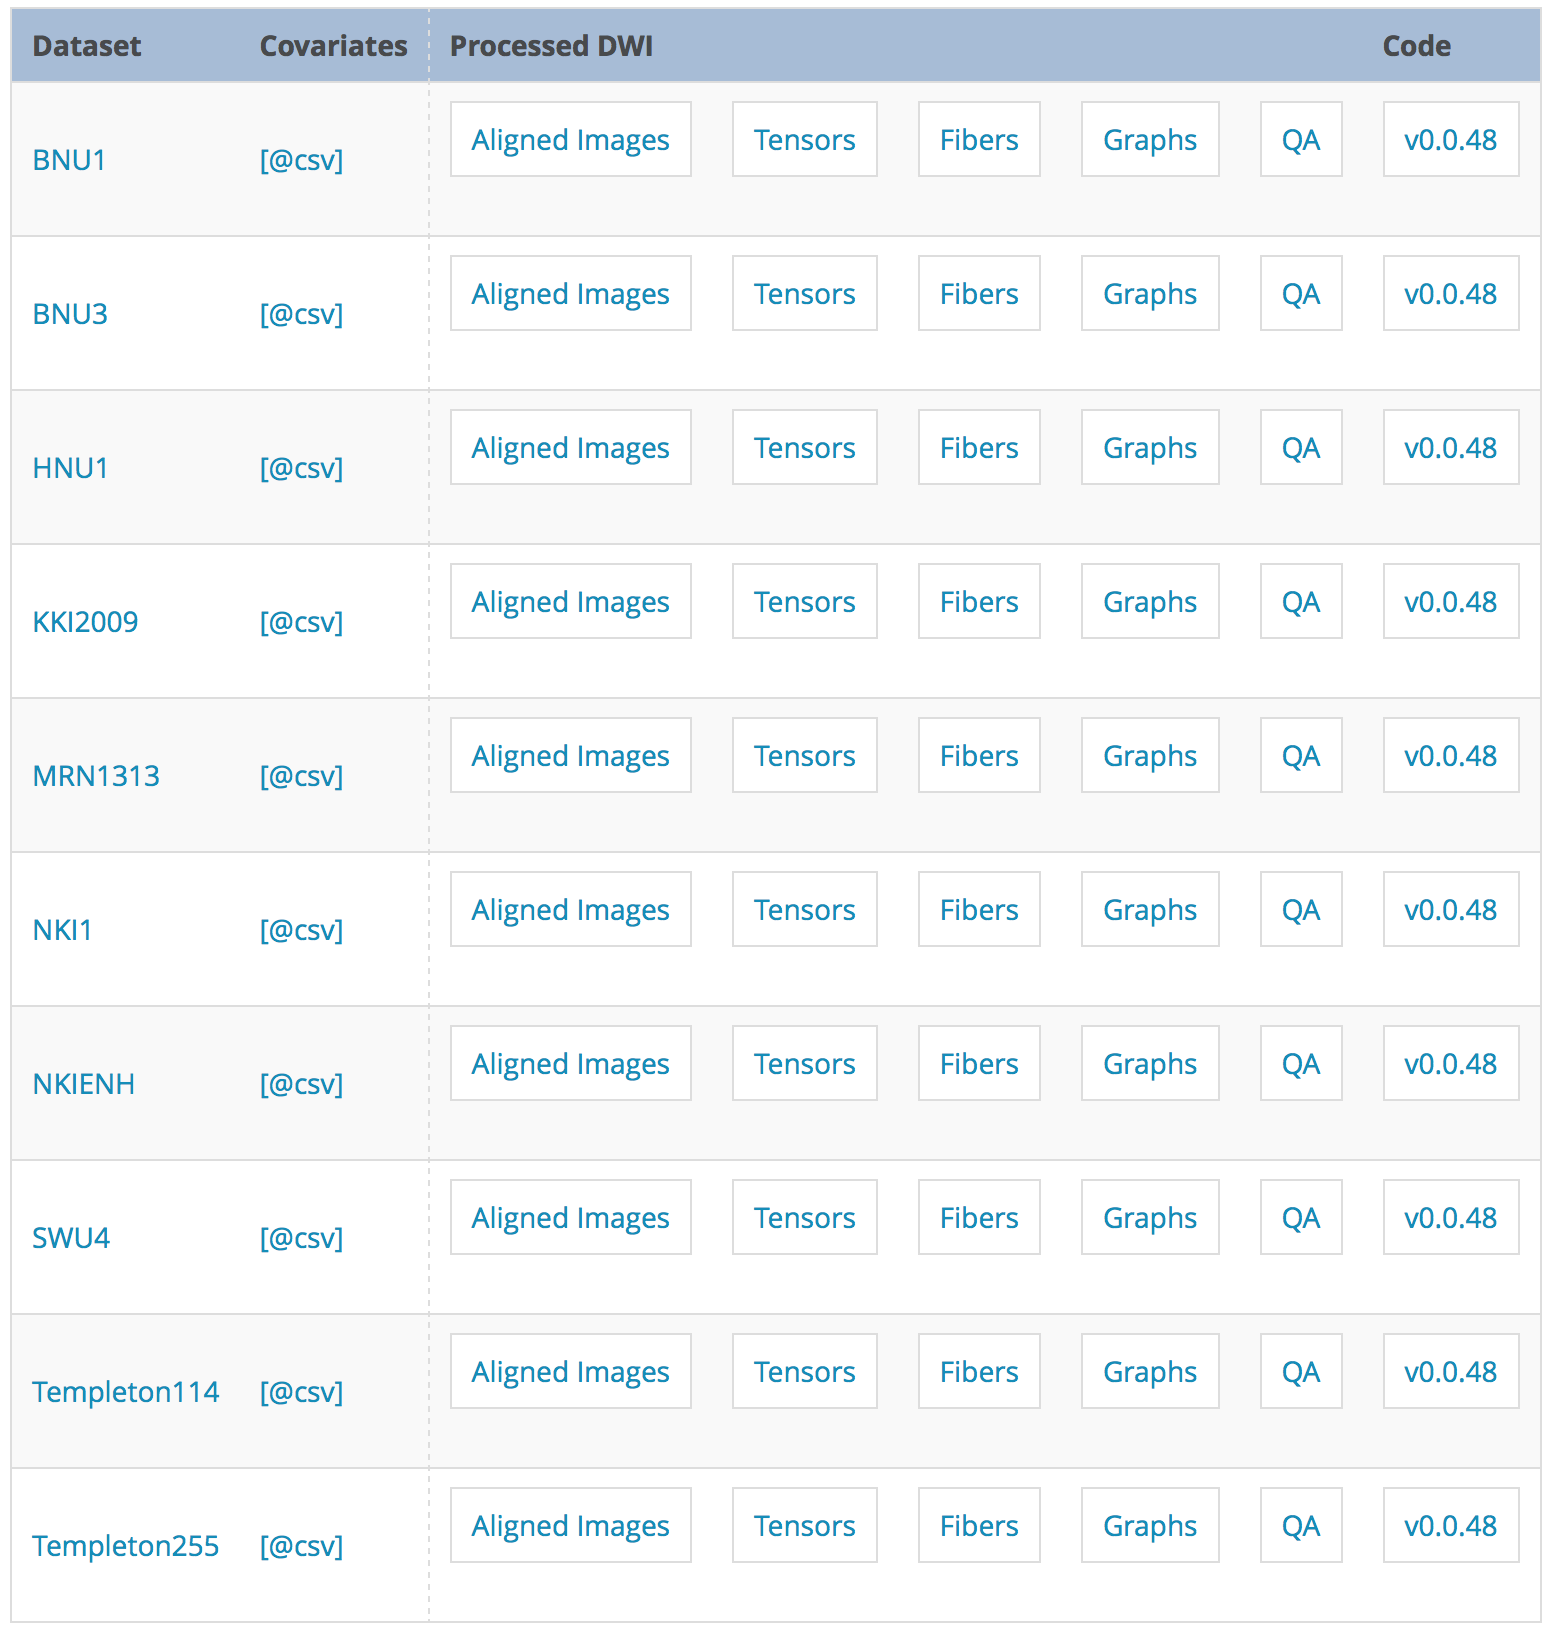
\includegraphics[height=0.65\textheight]{../../figs/DiffusionMRI_data201704.png}
\caption{A current snapshot of the diffusion magnetic resonance imaging data resulting from the pipeline \href{http://m2g.io}{m2g} for generating human connectomes at scale.}
\label{fig:dmri_data201704}
\end{cframed}
\end{figure}

\clearpage
\end{document}
